\documentclass[aspectratio=169,xcolor=dvipsnames]{beamer}

\usepackage{amsthm}
\usepackage{amsmath}
\usepackage{amssymb}
\usepackage{tikz}
\usepackage{pgfplots}
\usepackage{xfp}
\pgfplotsset{compat=1.18}
\usepackage[authoryear, round]{natbib}
\usepackage{hyperref}
\usetikzlibrary{arrows.meta,positioning,decorations.pathreplacing}
\hypersetup{
    colorlinks=true,
    linkcolor=blue,
    citecolor=blue,
    urlcolor=blue
}

\definecolor{darkgreen}{rgb}{0,0.5,0}
\definecolor{darkblue}{rgb}{0,0,0.55}

\newtheorem{proposition}{Proposition}
\setbeamertemplate{footline}[frame number]
\usetheme{Frankfurt}
\usefonttheme{serif}

\title{ECON8037: Financial Economics}
\subtitle{\normalsize Week 3 Lecture - Asset Valuation}
\author{Simon Mishricky}
\institute{Research School of Economics, Australian National University}
\date{\today}

\begin{document}

\section{CCAPM and Puzzles}
\frame{\titlepage}

\begin{frame}{CCAPM}
    We have the \textcolor{blue}{fundamental asset pricing equation} from the \textcolor{blue}{Consumption Capital Asset Pricing Model (CCAPM)}
    \[
        p_t = \mathbb{E}_t m_{t+1} g_{t+1}
    \]
    Where
    \[
        m_{t+1} = \beta \frac{u'(c_{t+1})}{u'(c_t)}, \quad g_{t+1} = y_{t+1} + p_{t+1}
    \]
    We have already shown how to derive this equation from the Lucas asset tree model.
\end{frame}

\begin{frame}{Mehra and Prescott}
    We can use the \textcolor{blue}{fundamental asset pricing equation} to derive the following equations from \textcolor{blue}{Mehra and Prescott (1985)}, which we will see in tutorials
    \begin{align*}
        r^f_{t+1} &= -\ln \beta + \gamma g - \frac{(\gamma \sigma)^2}{2} \\
        \mathbb{E}_t\left[r_{t+1} - r^f_{t+1}\right] &= \gamma \sigma \mathrm{cov}(r_{t+1}, \xi_{t+1}) - \frac{1}{2}\mathrm{var}(r_{t+1})
    \end{align*}
    Where $r_{t+1} = \ln(R_{t+1})$. Two famous puzzles emerge when we try to take these equations to data.
\end{frame}

\begin{frame}{Equity Premium Puzzle}
    \textcolor{blue}{Mehra and Prescott (1985)} implement the above CCAPM model empirically and find that an implausibly large risk aversion parameter is required to explain the equity premium relative to bonds in the US data. This is known as the \textcolor{blue}{Equity Premium Puzzle}.

    However, \textcolor{blue}{Weil (1989)} found that increasing the risk aversion parameter to the extent required to fit the equities data implies a large risk free rate. This is known as the \textcolor{blue}{Risk-Free Rate Puzzle}.
\end{frame}

\section{Asset Pricing Implications}

\begin{frame}{Asset Valuation}
    If we take the \textcolor{blue}{fundamental asset pricing equation} and split the variables, and since we know that $g_{t+1}/p_t = R_{t+1}$ we can write
    \begin{align*}
        p_t &= \mathbb{E}_t m_{t+1} g_{t+1} \\
        1 &= \mathbb{E}_t m_{t+1} R_{t+1} \\
        1 &= \mathbb{E}_t m_{t+1} \mathbb{E}_t R_{t+1} + \mathrm{cov}(m_{t+1}, R_{t+1})
    \end{align*}
    Since $m_{t+1}$ and $R_{t+1}$ are not independent. Where $\mathbb{E}_t m_{t+1} \mathbb{E}_t R_{t+1}$ is the time component and $\mathrm{cov}(m_{t+1}, R_{t+1})$ is the risk component. Given that $R^f_{t+1} = 1/\mathbb{E}_t m_{t+1}$
    \[
        1 = \frac{\mathbb{E}_t R_{t+1}}{R^f_{t+1}} + \mathrm{cov}(m_{t+1}, R_{t+1})
    \]
    Which becomes
    \[
        \mathbb{E}_t R_{t+1} - R^f_{t+1} = -R^f_{t+1} \mathrm{cov}(m_{t+1}, R_{t+1})
    \]
\end{frame}

\begin{frame}{Asset Valuation}
    All assets have an expected return equal to the risk-free rate, plus a risk adjustment.

    Assets whose returns covary positively with consumption make consumption more volatile, and so must promise higher expected returns to induce investors to hold them.

    Conversely, assets that covary negatively with consumption, such as insurance, can offer expected returns lower than the risk-free rate, or even negative (net) expected returns.

    This result contains some important implications.
\end{frame}

\begin{frame}{Asset Valuation}
    We tend to think of `risky' assets as those with volatile payoffs, and that this volatility should be compensated for in the price. But, if this payoff is uncorrelated with the stochastic discount factor $m_{t+1}$, the asset receives \emph{no} risk correction to its price and pays an expected return equal to the risk-free rate. We can see that if
    \[
        \mathrm{cov}(m_{t+1}, R_{t+1}) = 0
    \]
    Then the price is
    \[
        p_t = \frac{\mathbb{E}_t g_{t+1}}{R^f_{t+1}}
    \]
    No matter how large the variance of $g_{t+1}$ is. This means that \emph{idiosyncratic} risk, uncorrelated with the stochastic discount factor, generates no premiums.
\end{frame}

\begin{frame}{Beta Pricing Model}
    Given the above equation, but for a single asset $i$
    \[
        \mathbb{E}_t R^i_{t+1} - R^f_{t+1} = -R^f_{t+1} \mathrm{cov}(m_{t+1}, R^i_{t+1})
    \]
    We can rewrite as
    \[
        \mathbb{E}_t R^i_{t+1} = R^f_{t+1} + \beta_{i,m} \lambda_m
    \]
    Where
    \[
        \beta_{i,m} = \frac{\mathrm{cov}(R^i_{t+1}, m_{t+1})}{\mathrm{var}(m_{t+1})}, \quad \text{and} \quad \lambda_m = -\frac{\mathrm{var}(m_{t+1})}{\mathbb{E}_t m_{t+1}}
    \]
    This is known as the \textcolor{blue}{beta pricing model}.
\end{frame}

\begin{frame}{Beta Pricing Model}
    The \textcolor{blue}{beta pricing model} tells us that the expected return of an asset should be proportional to the $\beta_{i,m}$.

    Notice that $\lambda_m$ is the same for all assets $i$, while $\beta_{i,m}$ varies from asset to asset.

    $\lambda_m$ is interpreted as the price of risk and the $\beta_{i,m}$ as the quantity of risk in each asset. As you can see, the price of risk depends upon the volatility of the stochastic discount factor.
\end{frame}

\section{Mean-Variance Frontier}

\begin{frame}{Asset Valuation}
    Asset pricing theory has focused a lot on the means and variance of asset returns.

    Interestingly, the set of means and variances of returns is limited. All assets priced by the discount factor $m_{t+1}$ must obey (dropping the time subscripts)
    \[
        \left| \mathbb{E} R^i - R^f \right| \le \frac{\sigma(m)}{\mathbb{E} m} \sigma(R^i)
    \]
\end{frame}

\begin{frame}{Asset Valuation}
    To derive this result, take the \textcolor{blue}{fundamental asset pricing equation} for a given asset return $R^i$
    \begin{align*}
        1 &= \mathbb{E} m R^i \\
          &= \mathbb{E} m \mathbb{E} R^i + \mathrm{cov}(m, R^i) \\
          &= \mathbb{E} m \mathbb{E} R^i + \rho_{m, R^i} \sigma(R^i) \sigma(m)
    \end{align*}
    Since we know that $R^f = 1/\mathbb{E} m$, we can rewrite
    \[
        \mathbb{E} R^i = R^f - \rho_{m, R^i} \frac{\sigma(m)}{\mathbb{E} m} \sigma(R^i)
    \]
    And since correlation coefficients cannot be greater than 1, this implies
    \[
        \left| \mathbb{E} R^i - R^f \right| \le \frac{\sigma(m)}{\mathbb{E} m} \sigma(R^i)
    \]
\end{frame}

\begin{frame}{Asset Valuation}
    This inequality delineates the \textcolor{blue}{mean-variance frontier} and it has many important implications. Evidently, points on the frontier correspond to gross returns that are perfectly correlated (either positively and negatively) with the stochastic discount factor $m$. We summarise this as
    \[
        \rho_{m, R^i} = \begin{cases} +1 \implies R^i \text{ is on lower frontier} \\ -1 \implies R^i \text{ is on upper frontier} \end{cases}
    \]
\end{frame}

\begin{frame}{Mean-Variance Frontier}
    \centering
    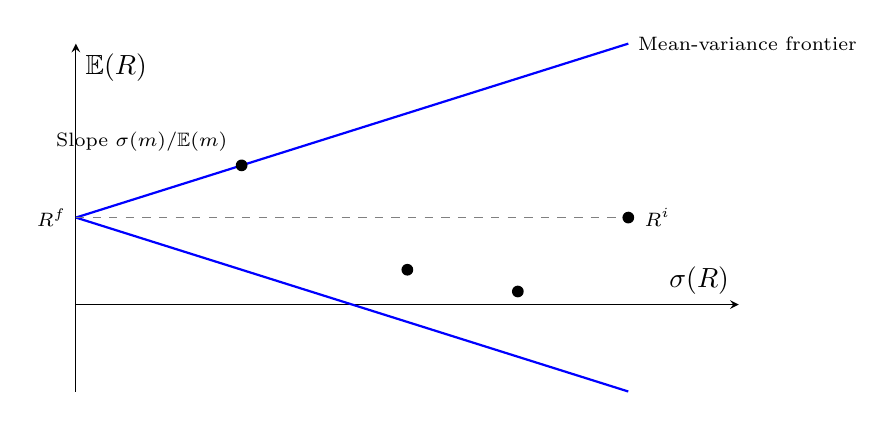
\begin{tikzpicture}
        \begin{axis}[
            width=10cm, height=6cm,
            xlabel={$\sigma(R)$}, ylabel={$\mathbb{E}(R)$},
            xmin=0, xmax=6, ymin=-2, ymax=6,
            axis lines=middle,
            xtick=\empty, ytick=\empty,
            clip=false
        ]
        % Upper frontier
        \addplot[blue, thick, domain=0:5] {2 + 0.8*x};
        % Lower frontier
        \addplot[blue, thick, domain=0:5] {2 - 0.8*x};
        % Idiosyncratic risk dashed
        \addplot[dashed, gray, domain=0:5] {2};
        % Some asset returns
        \node[circle,fill,inner sep=1.5pt,label=right:{\scriptsize $R^i$}] at (axis cs:5,2) {};
        \node[circle,fill,inner sep=1.5pt] at (axis cs:3,0.8) {};
        \node[circle,fill,inner sep=1.5pt] at (axis cs:4,0.3) {};
        \node[circle,fill,inner sep=1.5pt,label=above left:{\scriptsize Slope $\sigma(m)/\mathbb{E}(m)$}] at (axis cs:1.5,3.2) {};
        \node[anchor=east] at (axis cs:0,2) {\scriptsize $R^f$};
        \node[anchor=west] at (axis cs:5,6) {\scriptsize Mean-variance frontier};
        \end{axis}
    \end{tikzpicture}\\
    \footnotesize \textit{Figure 1.1.} Mean-variance frontier. The mean and standard deviation of all assets priced by a discount factor $m$ must lie in the wedge-shaped region.
\end{frame}

\begin{frame}{Asset Valuation}
    The structure of the mean-variance frontier implies that:

    \textbf{1. All returns on the frontier are perfectly correlated}

    Thus, let $R^m, R^{mv}$ be two returns on the frontier. Then for some scalar $a$, a return $R^{mv}$ on the mean-variance frontier satisfies the affine equation $R^{mv} = R^f + a(R^m - R^f)$. This is an exact equation with no residual.
\end{frame}

\begin{frame}{Asset Valuation}
    \textbf{2. Each return $R^{mv}$ on the mean-variance frontier is perfectly correlated with $m$}
    \[
        (\rho_{m, R^i} = -1) \implies \begin{cases} m = a + b R^{mv} \\ R^{mv} = e + dm \end{cases} \quad \text{for some scalars } a, b, e, d
    \]
    Therefore, any return on the mean-variance frontier is a legitimate discount factor.
\end{frame}

\begin{frame}{Asset Valuation}
    \textbf{3. For any mean-variance efficient return $R^{mv}$ that is on the frontier but that is not $R^f$, there exists a single-beta representation for any return $R^i$ that takes the form}
    \[
        \mathbb{E} R^i = R^f + \beta_{i, R^{mv}} \left[ \mathbb{E} R^{mv} - R^f \right]
    \]
    You may recognise this single-beta representation as the classic \textcolor{blue}{Capital Asset Pricing Model (CAPM)}.
\end{frame}

\begin{frame}{Asset Valuation}
    The essence of the \textcolor{blue}{beta pricing model} is that, even though the means and standard deviations of returns fill out the space inside the mean-variance frontier, a graph of mean returns versus \emph{beta} should yield a straight line.

    Since the beta model applies to every return including $R^{mv}$ itself, and $R^{mv}$ has a beta of 1 on itself, we can identify the factor risk premium as $\lambda = \mathbb{E}[R^{mv} - R^f]$. The last two points suggest an intimate relationship between discount factors, beta model, and mean-variance frontiers.
\end{frame}

\section{Sharpe Ratio and HJ Bound}

\begin{frame}{Asset Valuation}
    If we rearrange the inequality that characterises the mean-variance frontier, then we get
    \[
        \left| \frac{\mathbb{E} R^i - R^f}{\sigma(R^i)} \right| \le \frac{\sigma(m)}{\mathbb{E} m}
    \]
    The ratio of mean excess return to standard deviation
    \[
        \frac{\mathbb{E} R^i - R^f}{\sigma(R^i)}
    \]
    is known as the \textcolor{blue}{Sharpe ratio}. It is a common measure of risk-adjusted return.
\end{frame}

\begin{frame}{Asset Valuation}
    The \textcolor{blue}{Sharpe ratio} is a more interesting characterisation of an asset than the mean return alone.

    If you borrow and put more money into an asset, you can increase the mean return of the position, but you do not increase the \textcolor{blue}{Sharpe ratio}, since the standard deviation increases at the same rate as the mean.

    We can see that the \textcolor{blue}{Sharpe Ratio} is limited by the volatility of the stochastic discount factor. The maximal risk-return trade-off is steeper if there is more risk or more risk aversion.
\end{frame}

\begin{frame}{Asset Valuation}
    This formula is another way to capture the \textcolor{blue}{Equity Premium Puzzle}, and it suggests that either people are very risk averse, or that the stock returns of the last 50 years were good luck which will not continue.
\end{frame}

\begin{frame}{Asset Valuation}
    The slope of the mean-standard deviation frontier is the largest available \textcolor{blue}{Sharpe ratio}, and thus is naturally interesting. Let $R^{mv}$ again denote the return of a portfolio on the frontier, therefore the slope of the frontier is
    \[
        \left| \frac{\mathbb{E} R^{mv} - R^f}{\sigma(R^{mv})} \right| = \frac{\sigma(m)}{\mathbb{E} m} = \sigma(m) R^f
    \]
    Thus, the slope of the frontier is governed by the volatility of the stochastic discount factor. Which implies that the slope of the mean-variance frontier is higher if the economy is riskier --- if consumption is more volatile --- or if investors are more risk averse.

    Both situations also raise the slope of the expected return-beta line of the consumption beta model. Conversely, in an economy with a high \textcolor{blue}{Sharpe ratio}, low risk-aversion investors should take on so much risk that their consumption becomes volatile.
\end{frame}

\begin{frame}{Asset Valuation}
    Now returning to the expression that we derived earlier
    \[
        \left| \frac{\mathbb{E} R^i - R^f}{\sigma(R^i)} \right| \le \frac{\sigma(m)}{\mathbb{E} m}
    \]
    This restriction has become known as the \textcolor{blue}{Hansen-Jagannathan (HJ) bound}. The strength of the HJ bound lies in separating observable properties of returns on the left-hand side from the properties of the stochastic discount factor $m$.
\end{frame}

\begin{frame}{Asset Valuation}
    The \textcolor{blue}{Hansen-Jagannathan (HJ) bound} has to hold for all stochastic discount factors that prices return on the left-hand side, regardless of their economic foundations. And as we have seen above the bound effectively states that the \textcolor{blue}{Sharpe ratio} constitutes a lower bound on the volatility of the stochastic discount factor.

    This is a reframing of the statement above, i.e. ``the slope of the mean-standard deviation frontier is the largest available \textcolor{blue}{Sharpe ratio}''. Instead of asking what is the largest \textcolor{blue}{Sharpe ratio}, we can instead ask what is the lowest stochastic discount factor volatility.
\end{frame}

\begin{frame}{Asset Valuation}
    When framed in this way we can test out different stochastic discount factors. It turns out that contemporaneous models of stochastic discount factors which parameters deemed plausible missed the bound by a factor of ten or more, even for the most generic returns e.g. aggregate market portfolios.

    This has led to a substantial rethinking of approaches to stochastic discount factor modelling as large classes of models with low volatility of the stochastic discount factors could be discarded as implausible from the outset. Further highlighting the equity premium puzzle.
\end{frame}

\section{Recursive Utilities}

\begin{frame}{Asset Valuation}
    A number of solutions have been proposed to address both the equity premium puzzle and the risk-free rate puzzle, all of which contain issues. Below is a list of candidate solutions for these puzzles, some of which we will cover in this course
    \begin{itemize}
        \item Recursive utilities
        \item Liquidity
        \item Habit persistence
        \item Incomplete markets
        \item Leverage
    \end{itemize}
\end{frame}

\begin{frame}{Recursive Utilities}
    Knowing as we do that something is missing from our model, we must again conclude that the fundamental pricing equation is too simplistic. One idea is to modify our asset pricing equation in the following way
    \[
        p_t = \mathbb{E}_t \kappa_{t+1} m_{t+1} g_{t+1}
    \]
    Again, incorporating $\kappa_{t+1}$ does not tell us much until we endogenise this variable.
\end{frame}

\begin{frame}{Recursive Utilities}
    So far, we have supposed that the agents in our model know the objective probabilities of the exogenous processes that they face. This proposition relates to the idea of rational expectations. However, there are some complications to this idea, see the Ellsberg paradox.

    If we relax this idea and suppose that agents are uncertain about the probabilities they face. In this circumstance the agent must choose a probability distribution with which to make decisions with. This probability distribution can be chosen in a number of ways.
\end{frame}

\begin{frame}{Recursive Utilities}
    Consider an agent who chooses the distribution which they use to take expectations. This agent chooses a distribution that maximises the expectation whilst maintaining as much similarity as possible to the original distribution. To do this we replace the expectations operator in the agents problem with the following
    \[
        \rho(X) = \min_{\psi \in \mathcal{P}} \left\{ \mathbb{E}_\psi X - \frac{1}{\gamma} H(\psi || \phi) \right\}
    \]
    Where $\phi$ is the original distribution and $H$ is the Kullback-Leibler divergence, which has the form
    \[
        H(\psi || \phi) = \int \ln \left( \frac{\phi(x)}{\psi(x)}\right) \phi(x) dx
    \]
    And it measures how one probability distribution $\psi$ differs from another reference one $\phi$.
\end{frame}

\begin{frame}{Recursive Utilities}
    We can show that $\rho$ can be represented as
    \[
        \rho(X) = -\frac{1}{\gamma} \ln \left( \int e^{-\gamma X} \phi(X) dX\right) = -\frac{1}{\gamma} \ln \left(\mathbb{E}_t [e^{-\gamma X}]\right)
    \]
    Embedding this into the recursive formulation of the \textcolor{blue}{Lucas Jr (1978)} model, we get
    \[
        v_t(\pi_t, y_t) = \max_{\pi_{t+1}} \{ u(c_t) + \beta \rho(v_{t+1}(\pi_{t+1}, y_{t+1}))\}
    \]
    Subject to
    \[
        c_t + \pi_{t+1} p_t \le \pi_t y_t + \pi_t p_t, \quad c_t \ge 0 \quad 0 \le \pi_t \le 1 \text{ at each } t
    \]
\end{frame}

\begin{frame}{Recursive Utilities}
    Since the utility function is increasing, we know that the budget constraint binds. Substituting the budget constraint into the utility function, and replacing $\rho$, we have:
    \[
        v(\pi_t, y_t) = \max_{\pi_{t+1}} \left\{ u\left[\pi_t(y_t + p_t) - \pi_{t+1} p_t\right] - \frac{\beta}{\gamma} \ln \left( \mathbb{E}_t \left[ e^{-\gamma v(\pi_{t+1}, G(y_t, \xi_{t+1}))}\right]\right)\right\}
    \]
    Finding the first order condition, we get the pricing equation
    \[
        p_t = \mathbb{E}_t \kappa_{t+1} m_{t+1} g_{t+1}
    \]
    Where
    \[
        \kappa_{t+1} = \frac{e^{-\gamma v(\pi_{t+1}, G(y_t, \xi_{t+1}))}}{\mathbb{E}_t \left[ e^{-\gamma v(\pi_{t+1}, G(y_t, \xi_{t+1}))}\right]}, \quad m_{t+1} = \beta \frac{u'(c_{t+1})}{u'(c_t)}, \quad g_{t+1} = y_{t+1} + p_{t+1}
    \]
\end{frame}

\begin{frame}[allowframebreaks]{References}
    \small
    \begin{thebibliography}{99}
        \bibitem[Lucas Jr.(1978)]{lucas1978}
            Lucas Jr., R.\ E.\ Asset prices in an exchange economy. \textit{Econometrica: Journal of the Econometric Society}, pages 1429--1445, 1978.
        \bibitem[Mehra and Prescott(1985)]{mehra1985}
            Mehra, R.\ and E.\ C.\ Prescott. The equity premium: A puzzle. \textit{Journal of Monetary Economics}, 15(2):145--161, 1985.
        \bibitem[Weil(1989)]{weil1989}
            Weil, P.\ The equity premium puzzle and the risk-free rate puzzle. \textit{Journal of Monetary Economics}, 24(3):401--421, 1989.
    \end{thebibliography}
\end{frame}

\end{document}
